
%
%  void-input - easy report template for included file
%  EDIT THE LINE ABOVE FOR DOCUMENTATION OF THIS FILE, then delete this line! 
%         

%

% ============================================================
% --- texstudio magic comment: 
% !TEX encoding = UTF-8
% !TeX program = pdflatex
%% !TeX program = xelatex
% !TeX root = "cognome-tesina.tex"
% %  !TeX spellcheck = en_US
% !TeX spellcheck = it_IT


% ====================================================================


\chapter{Task 1}
The experience with this task has proved to be extremely advantageous as a first approach to pattern matching. After carefully selecting the method to use, I proceeded to determine the minimum distance between the points of the two images under control. Next, I narrowed down the range of points considered and verified that a minimum number of features fell within a pre-set threshold. Only in the presence of these conditions, I was able to confirm the effective correspondence between the two images. It should be emphasized that while the accuracy is not entirely perfect, it is remarkably close to 90\%. To have a better understanding of the result obtained, I invite you to take a look at the images below which show the photos with the relative matches identified. The Figure \ref{fig:1a}, Figure \ref{fig:1b} and Figure \ref{fig:1c}.

\begin{figure}[h]
	\centering
        \begin{minipage}{0.9\textwidth}
        		\centering
		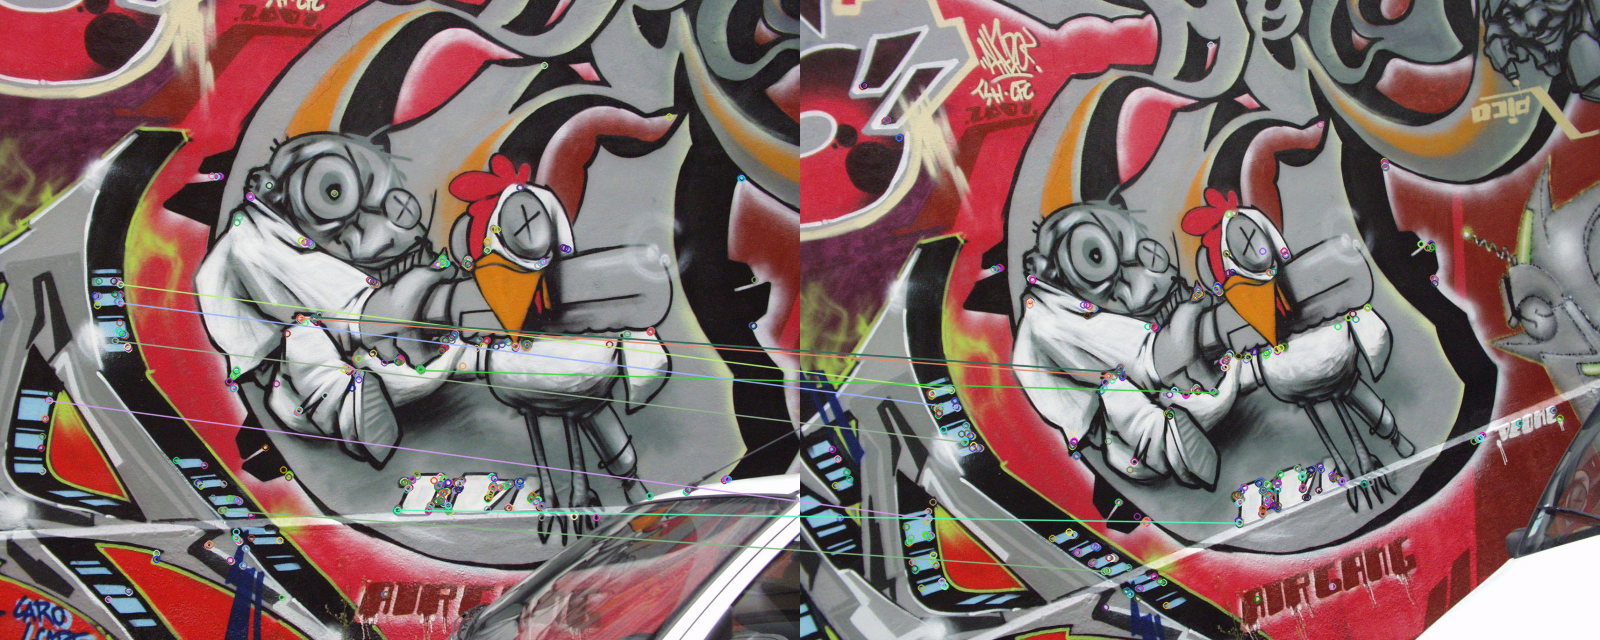
\includegraphics[width=\linewidth]{images/source/1}
		\caption{First image}
		\label{fig:1a}
        \end{minipage}
\end{figure}


\begin{figure}[h]
	\centering
        \begin{minipage}{0.9\textwidth}
        		\centering
		
\includegraphics[width=\linewidth]{images/source/2}
		\caption{Second image}
		\label{fig:1b}
        \end{minipage}
\end{figure}


\begin{figure}[h]
	\centering
        \begin{minipage}{0.9\textwidth}
        		\centering
		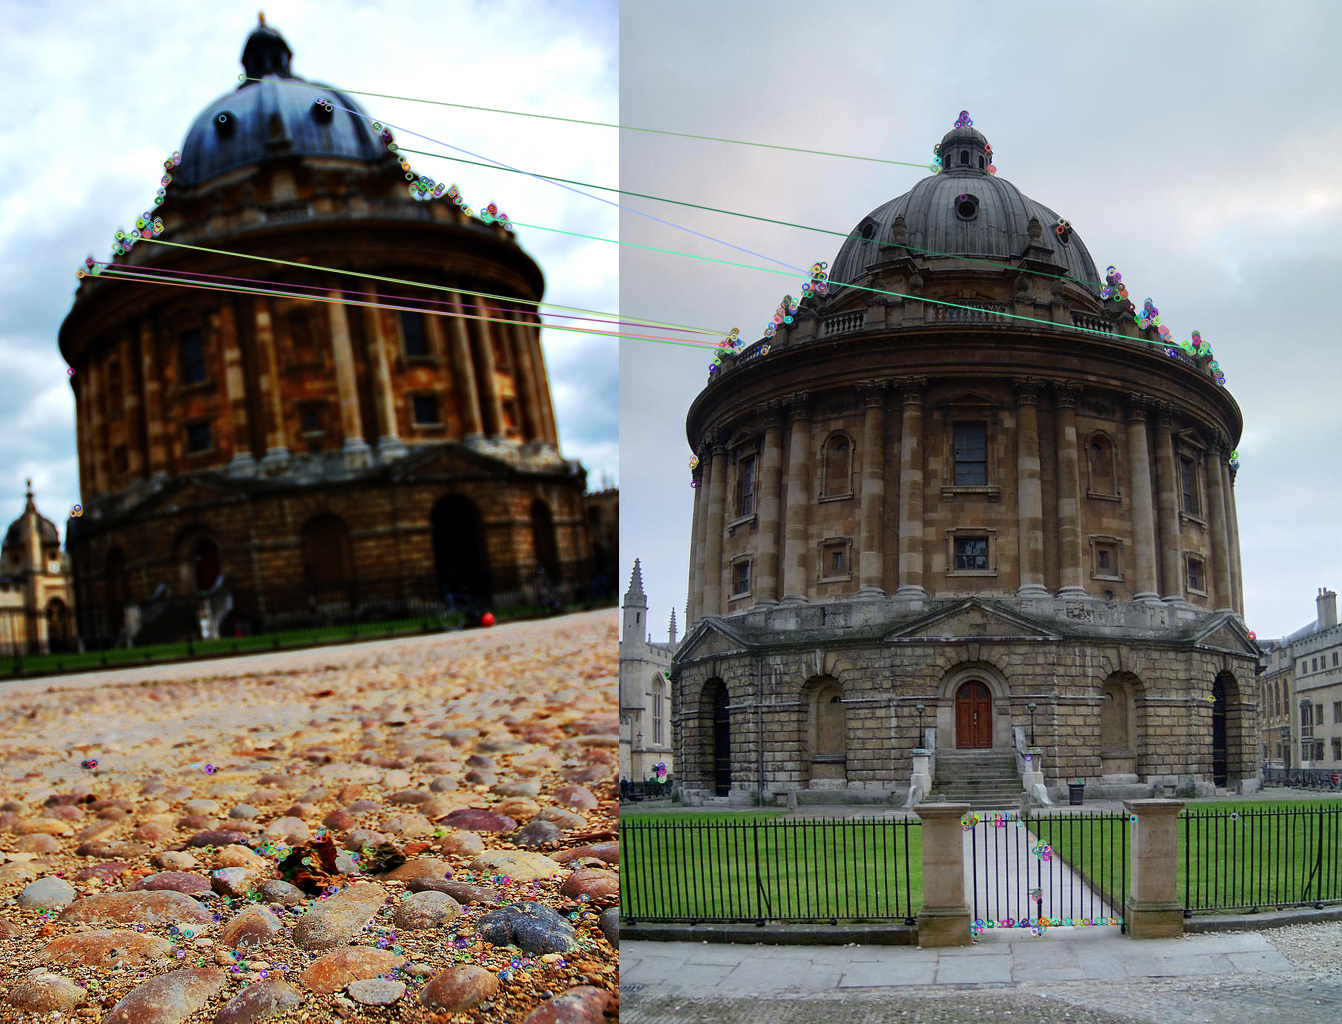
\includegraphics[width=\linewidth]{images/source/3}
		\caption{Third image}
		\label{fig:1c}
        \end{minipage}
\end{figure}

% ====================================================================

% ====================================================================
% memo available commands
% ====================================================================
% easyrep: summary of provided macros
%
% \Title{text}     defines the document title 
% \Subtitle{text}  defines the subtitle
% \Author{text}    defines the author string
% \Date{text}      defines a date string
% \printCover      print a cover page using above information
%
% --- text styles
% \tDef{text}      definition (generic) 
% \tDefObj{text}   definition (the ter being defined)
% \tDefTxt{text}   definition (the statement defining the term) 
% \tRemark{text}   remarked text
% \tREMARK{text}   highly remarked text 
% \tLoud{text}     shouted text! 
% \tCode{text}     inline code text
% \tLatin{text}    latin text
% \tForeign{text}  foreign language text 
% \tExample{text}  example 
% \tStandard{text} a recommendation 
% \tQuote{text}    a quoted text 
% \tQuoteFig{text} a quoted text referring to a figure 
% \tConcept{text}  an important concept  
% \tBeginPar{text} highlighted text 
%                  at the beginning of a paragraph 
%
% ---environments
% \begin{quoteStandard} text... \end{quoteStandard}
%    print text to be quoted, e.g. sentences from 
%    a recommendation
%
% \begin{quoteRemark} text... \end{quoteRemark}
%    similar to quoteStandrd, but the text is more marked
%
%  
% --- typo accelerators
% \qmo             opening quotation mark (use \qmo{})
% \qmc             closing quotation mark (use \qmc{})
% \th  emphasises "th"
% \ie  slanted "i.e."
% \eg  slanted "e.g."
% \es  slanteg "ad es."
% \octave   "octave" in \tCode style
% \matlab   "matlab"
% \labview  "labVIEW"
% \latex    "LaTeX" (just the text!)
%
% --- math typo accelerators
% \v{math text}  underlines the math text (useful for vector) 
%
% --- debug commands
% \debugTextStyles        print a table showing text styles
% \debugPrintCharacters   print a table of characters
% \Vispa                  print some text (to fill)  
% \Vispas                 more filling text
% ====================================================================
